%Arc Flash Report

\documentclass{article}
\usepackage{graphicx}
\usepackage[pdftex,bookmarks,bookmarksnumbered,colorlinks]{hyperref}
\usepackage{pdfpages}
\usepackage{fancyhdr}
\usepackage[english]{babel}
\usepackage{multicol}
\usepackage[margin=1.1in]{geometry}
\usepackage{textcomp}
\usepackage{fmtcount}
\usepackage[utf8]{inputenc}
\usepackage{hyperref}

%Prevents Tables from being repositioned
\usepackage{float}
\restylefloat{table}

% Table spacing
%Top space
\newcommand{\Toprule}{\rule{0pt}{3.0ex}}
%Bottom space
\newcommand{\Botrule}{\rule[-1.2ex]{0pt}{0pt}}

%Constants
\newcommand{\DocTitle}{ARC FLASH HAZARD ANALYSIS}
\newcommand{\Customer}{Fanshawe College}
\newcommand{\Building}{Main Campus}
\newcommand{\Address}{1001 Fanshawe College Blvd}
\newcommand{\JobNum}{S2940\_01}


%hyperlinks
\hypersetup{
pdftoolbar=true,        								% show Acrobat�s toolbar?
pdfmenubar=true,        								% show Acrobat�s menu?
pdffitwindow=false,     								% window fit to page when opened
pdfstartview={FitH},    								% fits the width of the page to the window
pdftitle={\DocTitle},    								% title
pdfauthor={PowerCore Engineering},    	% author
pdfsubject={Report},   									% subject of the document
pdfcreator={PowerCore Engineering},   	% creator of the document
pdfproducer={PowerCore Engineering}, 		% producer of the document
pdfnewwindow=true,      								% links in new window
colorlinks=true,       									% false: boxed links; true: colored links
linkcolor=black,          							% color of internal links (change box color with linkbordercolor)
citecolor=blue,        									% color of links to bibliography
filecolor=blue,      										% color of file links
urlcolor=blue}           								% color of external links


%Header and Footer
\renewcommand{\sectionmark}[1]{\markboth{#1}{}}
\renewcommand{\footrulewidth}{0.4pt}
\fancyhead[R]{\leftmark} % 1. sectionname
\fancyfoot[C]{\thepage}
\fancyfoot[L]{
PowerCore Engineering\\
London, Ontario, Canada\\
Tel: (519) 474-1175\\
\url{www.powercore.ca}}
\cfoot{ }

\fancyfoot[R]{
\DocTitle \\ \vspace{12pt}  -\thepage -}
\fancypagestyle{plain}{%
  \fancyhf{}%
  \renewcommand{\headrulewidth}{0pt}%
}
\fancyhead[L]{ % right
   
\includegraphics[height=0.4in]{Images/logo_SV3.PNG}
}

\begin{document}

\pagenumbering{Alph}
\begin{titlepage}
\thispagestyle{empty}
\center % Center everything on the page

%Title Page Header
\begin{center}

\includegraphics[height=1in, keepaspectratio=true]{../Images/PCEHeader.PNG}
\end{center}

%TITLE SECTION
\begin{center}
\vspace{20mm}
\Huge \DocTitle \\ % Title of your document
\vspace{75mm}
\large Prepared for: \\
\LARGE\textbf{\Customer} \\
\large\textbf{\Building}\\
\small\textbf{\Address}\\
\end{center}


%LOGO SECTION
%
\includegraphics[width=2.5in, keepaspectratio=true]{Images/logo_SV.png} 

 
%AUTHOR SECTION
\begin{flushleft} \large
\vfill

\textbf{Prepared by:} \\
Roman Bulla, P. Eng., Scott Vermeire, EIT \\
%Roman Bulla, P. Eng., Vince Klingenberger \\
\vspace{12pt} 
\textbf{Completion:}\\
\today \\ 
\vspace{12pt} 
\textbf{Job Number:}\\
\JobNum \\
\end{flushleft}

\end{titlepage}

\pagenumbering{arabic}
\pagestyle{fancy}

%TOC
\tableofcontents
\pagebreak


%Introduction
\section{Introduction}
\label{af:intro}

\subsection{Introduction to Project}
\label{af:intro:proj}

The Arc Flash Hazard Evaluation Study for \Customer{} was prepared by PowerCore Engineering.\\

The Arc Flash Hazard Evaluation Study determined: the Arcing Fault Clearing Time, Limits of Approach, Working Distance, Incident Energy, Clothing Requirements and Hazard Area Classifications for all electrical equipment within the scope of the study.\\

Arc Flash Study was performed in compliance with IEEE Std-1584-2002 and CSA Z462-15. The study was based on the short-circuit information and protective device settings provided by \Customer{}.

\subsection{Scope}
\label{af:intro:scope}

The study results shall be the basis for implementation of an Arc Flash Hazard Program, that will meet regulation NFPA 70E, CSA Z462 as well as IEEE-1584.\\





%Arc Flash Study Results & Recommendations

\section{Results}
\label{af:results}

\subsection{Arc Flash Study Results and Recommendations}
\label{af:results:afrr}

The Arc Flash Hazard Evaluation Study has shown that:

\pagebreak

\subsection{Arc Flash Study Details}
\label{af:results:afsd}

The following issues have been encountered and are of note:

\begin{itemize} 
\item The risk category for all downstream equipment from the last bus or power panel listed on the summary sheet and shown on the drawings shall be treated as the last indicated Hazard Category, unless indicated otherwise.

\item Arc Flash Hazard Identification labels for all equipment within the scope of this study will be affixed in a visible area.

\item Please note that the operation of fused switches or starters with cover on or enclosure doors closed does not require arc flash rated PPE Hazard, based on CSA Z462.

\item\textbf{Equipment below 240 V need not be considered (for Arc Flash Hazard Analysis) unless it involves at least one 125 kVA or larger low impedance transformer in its immediate power supply.}\cite{IEEE}	 
\end{itemize}
\pagebreak
\subsection{Study Recommendations}
\label{af:results:afsr}

Based on the Arc Flash evaluation Study performed, we recommend the following:
\begin{itemize}
\item We recommend that all personnel authorized to operate any electrical equipment be properly educated on Arc Flash Hazard and trained  in use of arc flash PPE (Personal Protective Equipment)

\item	Provide PPE of appropriate level to all personnel that will be operating electrical equipment.

\item	We recommend that a formal written Electrical Equipment Operation Procedures Manual as well as an Arc Flash Hazard Program that meets the regulations noted in CSA Z462-15 and IEEE-1584, be developed and implemented.
\end{itemize}
\vspace{10mm}
\noindent Thank you for this opportunity to be of service to you.  If you have any questions regarding the recommendations in this report or any other matter, please contact our London Engineering Services office at (519) 474-1175. \newline
\vspace{5mm}
\\
\noindent Sincerely,\newline

\vspace{5mm}
\noindent\textbf{PowerCore Engineering}\newline


\begin{multicols}{2}
\centering

\includegraphics[height=0.5in, keepaspectratio=true]{Images/Roman_signature.jpg} \\
Roman Bulla, P. Eng. \\Power Systems Engineer \\

\includegraphics[height=0.5in, keepaspectratio=true]{Images/Scott_signature.jpg} \\
Scott Vermeire \\Engineering Intern \\
\end{multicols}
%Objectives
\section{Objectives}
\label{af:o}

\subsection{Arc Flash Study Objectives}
\label{af:o:afso}

The study results shall be basis for implementation of an Arc Flash Hazard Program, that will meet regulation CSA Z462 as well as IEEE-1584.
\\
\\
Arc flash hazards can result from many factors, including dropped tools, accidental contact with electrical systems, build up of conductive dust, corrosion and improper work procedures. An arc is produced by flow of electrical current through ionized air after an initial flashover or short circuit, resulting in a flash that can cause significant heating and burn injuries to occur. 
\\
\\
Arc faults can cause serious injury or death to workers. At the initiation of an arc fault, tremendous energy can be released in a very brief time. Metal conductor parts can vaporize resulting in hot vapors and hot metal being violently spewed. The thermal energy can result in severe burns to workers caused by direct
exposure or clothing ignition.
\\
\\
Historically, the Electrical Safety Code and other safety codes have been primarily concerned with protection from fire, electrocution, and shock hazard.  Arc flash hazards were not addressed. This is changing.
\\
\\
Canadian Standards Association (CSA) Z462 standard and Institute of Electrical and Electronics Engineers (IEEE) 1584 2002, provide guidance on implementing appropriate safety procedures to limit Arc Flash Hazard.
\\
\\
OSHA considers CSA Z462 a consensus industry standard for assessing arc flash standards. Under this legislation, the employer is responsible to assess the hazards in the work place; Select, have, and use the correct PPE and Document the assessment.
\\
\\
OSHA considers Arc Flash assessments that follow CSA Z462, in compliance with OSHA requirements, and the accepted practice to protect workers from electrical safety hazards.
\\
\\
To implement a successful Arc Flash Hazard prevention program, an Arc Flash study shall be performed to in a manner that satisfies the regulation CSA Z462 as well as IEEE-1584.
\\
\\
For each selected location of your power distribution system, the Arc Flash analysis shall determine the Incident Energy, Arcing Fault Clearing Time; Limits of approach, 
Working Distance, Incident Energy, Clothing Class required and Hazard area classification.
\\
\\
The objective of the Analysis is to determine a number of factors that directly affect the Arc Flash Hazard:
\\
\\
\textbf{Incident Energy Exposure }\\   
This is the amount of thermal incident energy to which the worker's face and chest could be exposed at working distance during an electrical arc event. Incident energy is measured in joules per centimeter squared (J/cm2) or calories per centimeter squared (cal/cm2). 
\\
\\  
\textbf{Flash Protection Boundary }\\   
The flash protection boundary is an approach limit at a distance from exposed live parts or enclosed live parts if operation, manipulation, or testing of equipment creates a potential flash hazard, within which a person could receive a second degree burn if an electrical arc flash were to occur. A worker entering the flash protection boundary must be qualified and must be wearing appropriate PPE. The Flash Protection Boundary is required to be calculated by CSA Z462. 
\\
\\ 
\textbf{Level of PPE} \\   
This is the minimum level of Personal Protective Equipment in calories per centimeter squared, as evaluated in IEEE Standard 1584, with the intent to protect the worker from the thermal effects of the arc flash at 18 inches from the source of the arc.
\\
\\		
\textbf{Gap}\\
Gap between conductors where arc will occur.
\\
\\		
\textbf{Working Distance}\\
Closest distance to a worker's body excluding arms and hands, which would be exposed to the arc.
\\
\\		
\textbf{Clothing Class}\\
Minimum clothing class designed to protect a worker from second degree burns.
\\
\\
The following Table outlines the current standards:
\\
\begin{center}

\textbf{Minimum Thermal Recommended Protection}\\
(Based on CSA Z462 Table 5 pg. 47-48)

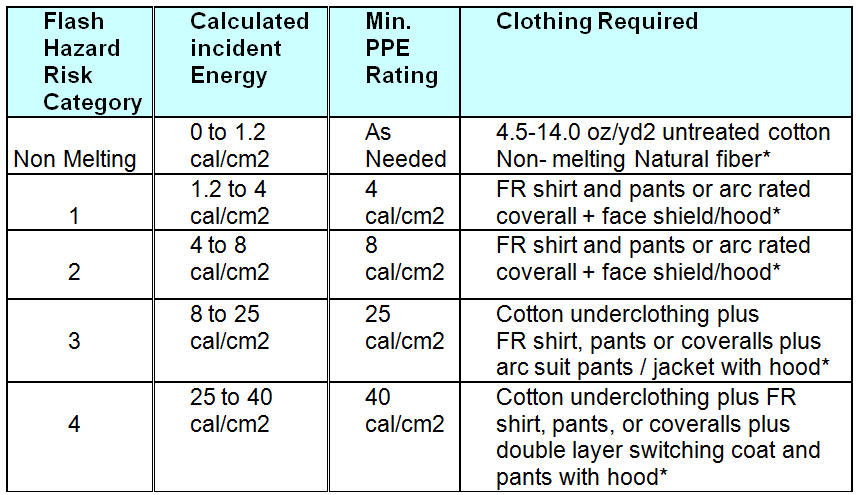
\includegraphics[width=5in, keepaspectratio=true]{../Images/Clothing.png} \\

\end{center}

\noindent *Note: In addition to clothing FR protective equipment is required as needed. Please see table 5 in CSA Z462 standard for further information. This can include items such as FR rated hard hats with inserts, safety glasses/goggles, hearing protection, leather safety shoes/gloves. Etc.

\pagebreak

\noindent The Arc Flash Analysis is merely a first step in implementing an Arc Flash Hazard Management Program.  The results of the study shall be further utilized in steps such as:\\

\begin{itemize}
\item	Implement the results of the Arc Flash Analysis - Modify your power distribution system parameters as needed (change settings on the protective relays/breakers, replace fuses etc.)
\\
\item	Implement a comprehensive labeling program - Identify all Electrical Equipment in the plant, including sources of power and limits of approach  
\\
\item	PPE and Training - Provide instructions and Personal Protective Equipment to all personnel that will be operating major electrical equipment.
\\
\item	Modify operating procedures (where practical) - change in switching arrangements, add remote tripping/closing to selected breakers, use long operating arms etc.
\end{itemize}
%Procedures
\section{Procedures}
\label{af:p}

\subsection{Arc Flash Study Procedures}
\label{af:p:afsp}

\emph{CSA Z462} focuses on safety and the way in which a worker plans and executes a task. When it's necessary to work on energized equipment, written work permits that include a description of the work to be done and the safety hazards involved should be issued. However, wearing the proper safety equipment for the risk hazard involved doesn't guarantee that a worker will remain free from injury or burns. Its purpose is to reduce deaths and life threatening burns.\\

The focus of \emph{IEEE Std. 1584} is the radiated heat or incident energy produced by an arcing fault that falls on a given surface. A bolted fault doesn't produce any radiated flash energy since no arc is involved. A value of 1.2 calorie/cm2 (1.2 calorie/cm2=5.02 Joules/cm2=5.02 Watt-sec/cm2) for a clearing time of 0.1 second is the incident energy level generally used as a guide to restrict the flash hazard to a second-degree or curable burn. In order to maintain that same level of injury, if the clearing time were increased to 1.0 second, the energy level would have to be reduced to 0.12 calorie/cm2.\\

To properly estimate the exposure hazard, it's necessary to have the maximum bolted short-circuit current, the arcing fault current, and the operating time of the interrupting device at the arcing fault current. The incident energy should be calculated at maximum and at 85\% of maximum arc fault current levels. Due to the inverse nature of protective devices, such as fuses and relays, a longer operating time at lower arcing currents can result in a higher energy exposure.\\

To model the power distribution system effectively, and to obtain as accurate results as possible, a number of parameter / factors have to be determined:\\ 

\noindent\textbf{Equipment Class } \\
\noindent Classes of equipment included in IEEE 1584 and typical bus gaps are shown in table below: 

\begin{center}
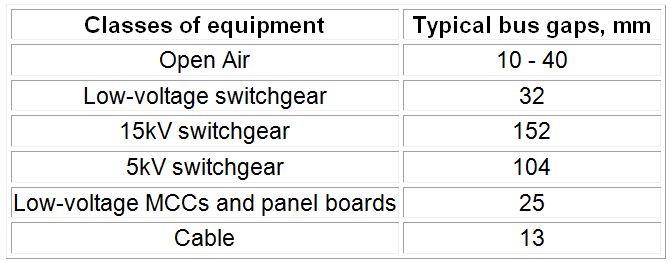
\includegraphics[width=5in, keepaspectratio=true]{../Images/Gaps.png} \\
\end{center}

\noindent\textbf{Gap between Conductors } \\  
\noindent Equipment bus gap in mm. Gaps of 3 to 40 mm are used for low voltage testing to simulate gaps between conductors in low voltage equipment and cables. Gaps 13, 104 and 152 mm. are used in 5 and 15kV equipment testing.\\
   
\noindent\textbf{Grounding Type}    \\
\noindent Two grounding classes are applied in the IEEE 1584 procedure, as follows:
\begin{enumerate}
	\item Ungrounded, this included ungrounded, high-resistance grounding and low-resistance grounding.
	\item Solidly grounded. 
\end{enumerate}

\noindent\textbf{Working Distance }  \\ 
\noindent Typical working distance is the sum of the distance between the workers standing in front of the equipment, and from the front of the equipment to the potential arc source inside the equipment. \\

\noindent Arc-flash protection is always based on the incident energy level on the person's face and body at the working distance, not the incident energy on the hands or arms. The degree of injury in a burn depends on the percentage of a person's skin that is burned. The head and body are a large percentage of total skin surface area and injury to these areas is much more life threatening than burns on the extremities. \\

\noindent Typical working distances are shown in table below:
\begin{center}
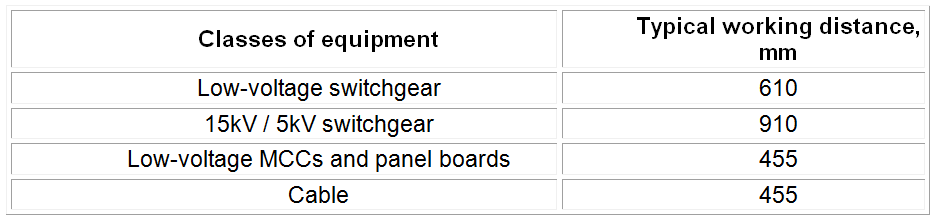
\includegraphics[width=5in, keepaspectratio=true]{../Images/WorkingDistance.png} \\
\end{center}

\noindent\textbf{Arc Duration / Total Clearing Time   } \\
\noindent Protective device characteristics, which can be found in the manufacturers, supplied data. For fuses, the manufacturer's time-current curves may include both melting and clearing time. In such a case, the clearing time is used. If they show only the average melt time, 15\% is added to that time, up to 0.03 seconds, and 10\% above 0.03 seconds to determine total clearing time. If the arcing fault current is above the total clearing time at the bottom of the curve (0.01 seconds), 0.01 seconds is used for the time. \\
For circuit breakers with integral trip units, the manufacturer's time-current curves include both tripping time and clearing time. \\

\noindent For relay operated circuit breakers, the relay curves show only the relay operating time in the time-delay region. For relays operating in their instantaneous region, 16 milliseconds are typically allowed on 60 Hz systems for operation. The circuit breaker opening time must be added. Opening times for particular circuit breakers can be verified by consulting the manufacturer's literature. \\
 
  
\noindent\textbf{Available 3 Phase Bolted Fault Current}  \\ 
Available 3 phase bolted fault current for each specific location as determined by the Short Circuit Analysis. \\
 
\noindent\emph{NOTE: Effect of arc current variation on determination of clearing time:    
For protective devices operating in the steep portion of their time-current curves, a small change in current causes a big change in operating time. Incident energy is linear with time, so arc current variation may have a big effect on incident energy. The solution is to make two arc current and energy calculations; one using the calculated expected arc current and one using a reduced arc current that is 15\% lower.}\\ 

%Observations
\section{Observations}
\label{af:observations}

\subsection{Arc Flash Hazard Study Detailed Results}
\label{af:observations:at}

Please refer to Arc Flash Report Table for detailed Arc Flash Analysis Results.

\pagebreak

\subsection{Power Distribution System Single Line Diagrams}
\label{af:observations:sld}

The following pages depict a detailed Equipment Single Line Diagram (SLD) and Arc Flash Hazard SLD.

\begin{thebibliography}{1}

\bibitem{IEEE} Institute of Electrical and Electronics Engineers {\em Std 1584: IEEE Guide for Performing Arc Flash Hazard Calculations}  2002.
\bibitem{CSA} CSA {\em Z462-15: Workplace Electrical Safety}  2015.
\bibitem{NFPA} NFPA {\em NFPA 70E: Standard for Electrical Safety in the Workplace and Handbook}  2015.
\bibitem{Doan} Doan {\em Arc Flash Calculations for Exposure to DC Systems. Transactions on Industry Applications, Vol. 46, No.5.}  2007.

\end{thebibliography}

\end{document}